%\begin{landspace}
%	\begin{multicols}{2}
%		\appendix\label{anhang:a}
%		\chapter{Anhang}
%		\section{Quell-Code}
%		% ---
%	\end{multicols}
%\end{landspace}

\appendix
\begin{landscape}
	\chapter{Anhang}\label{anhang:schaltung}
	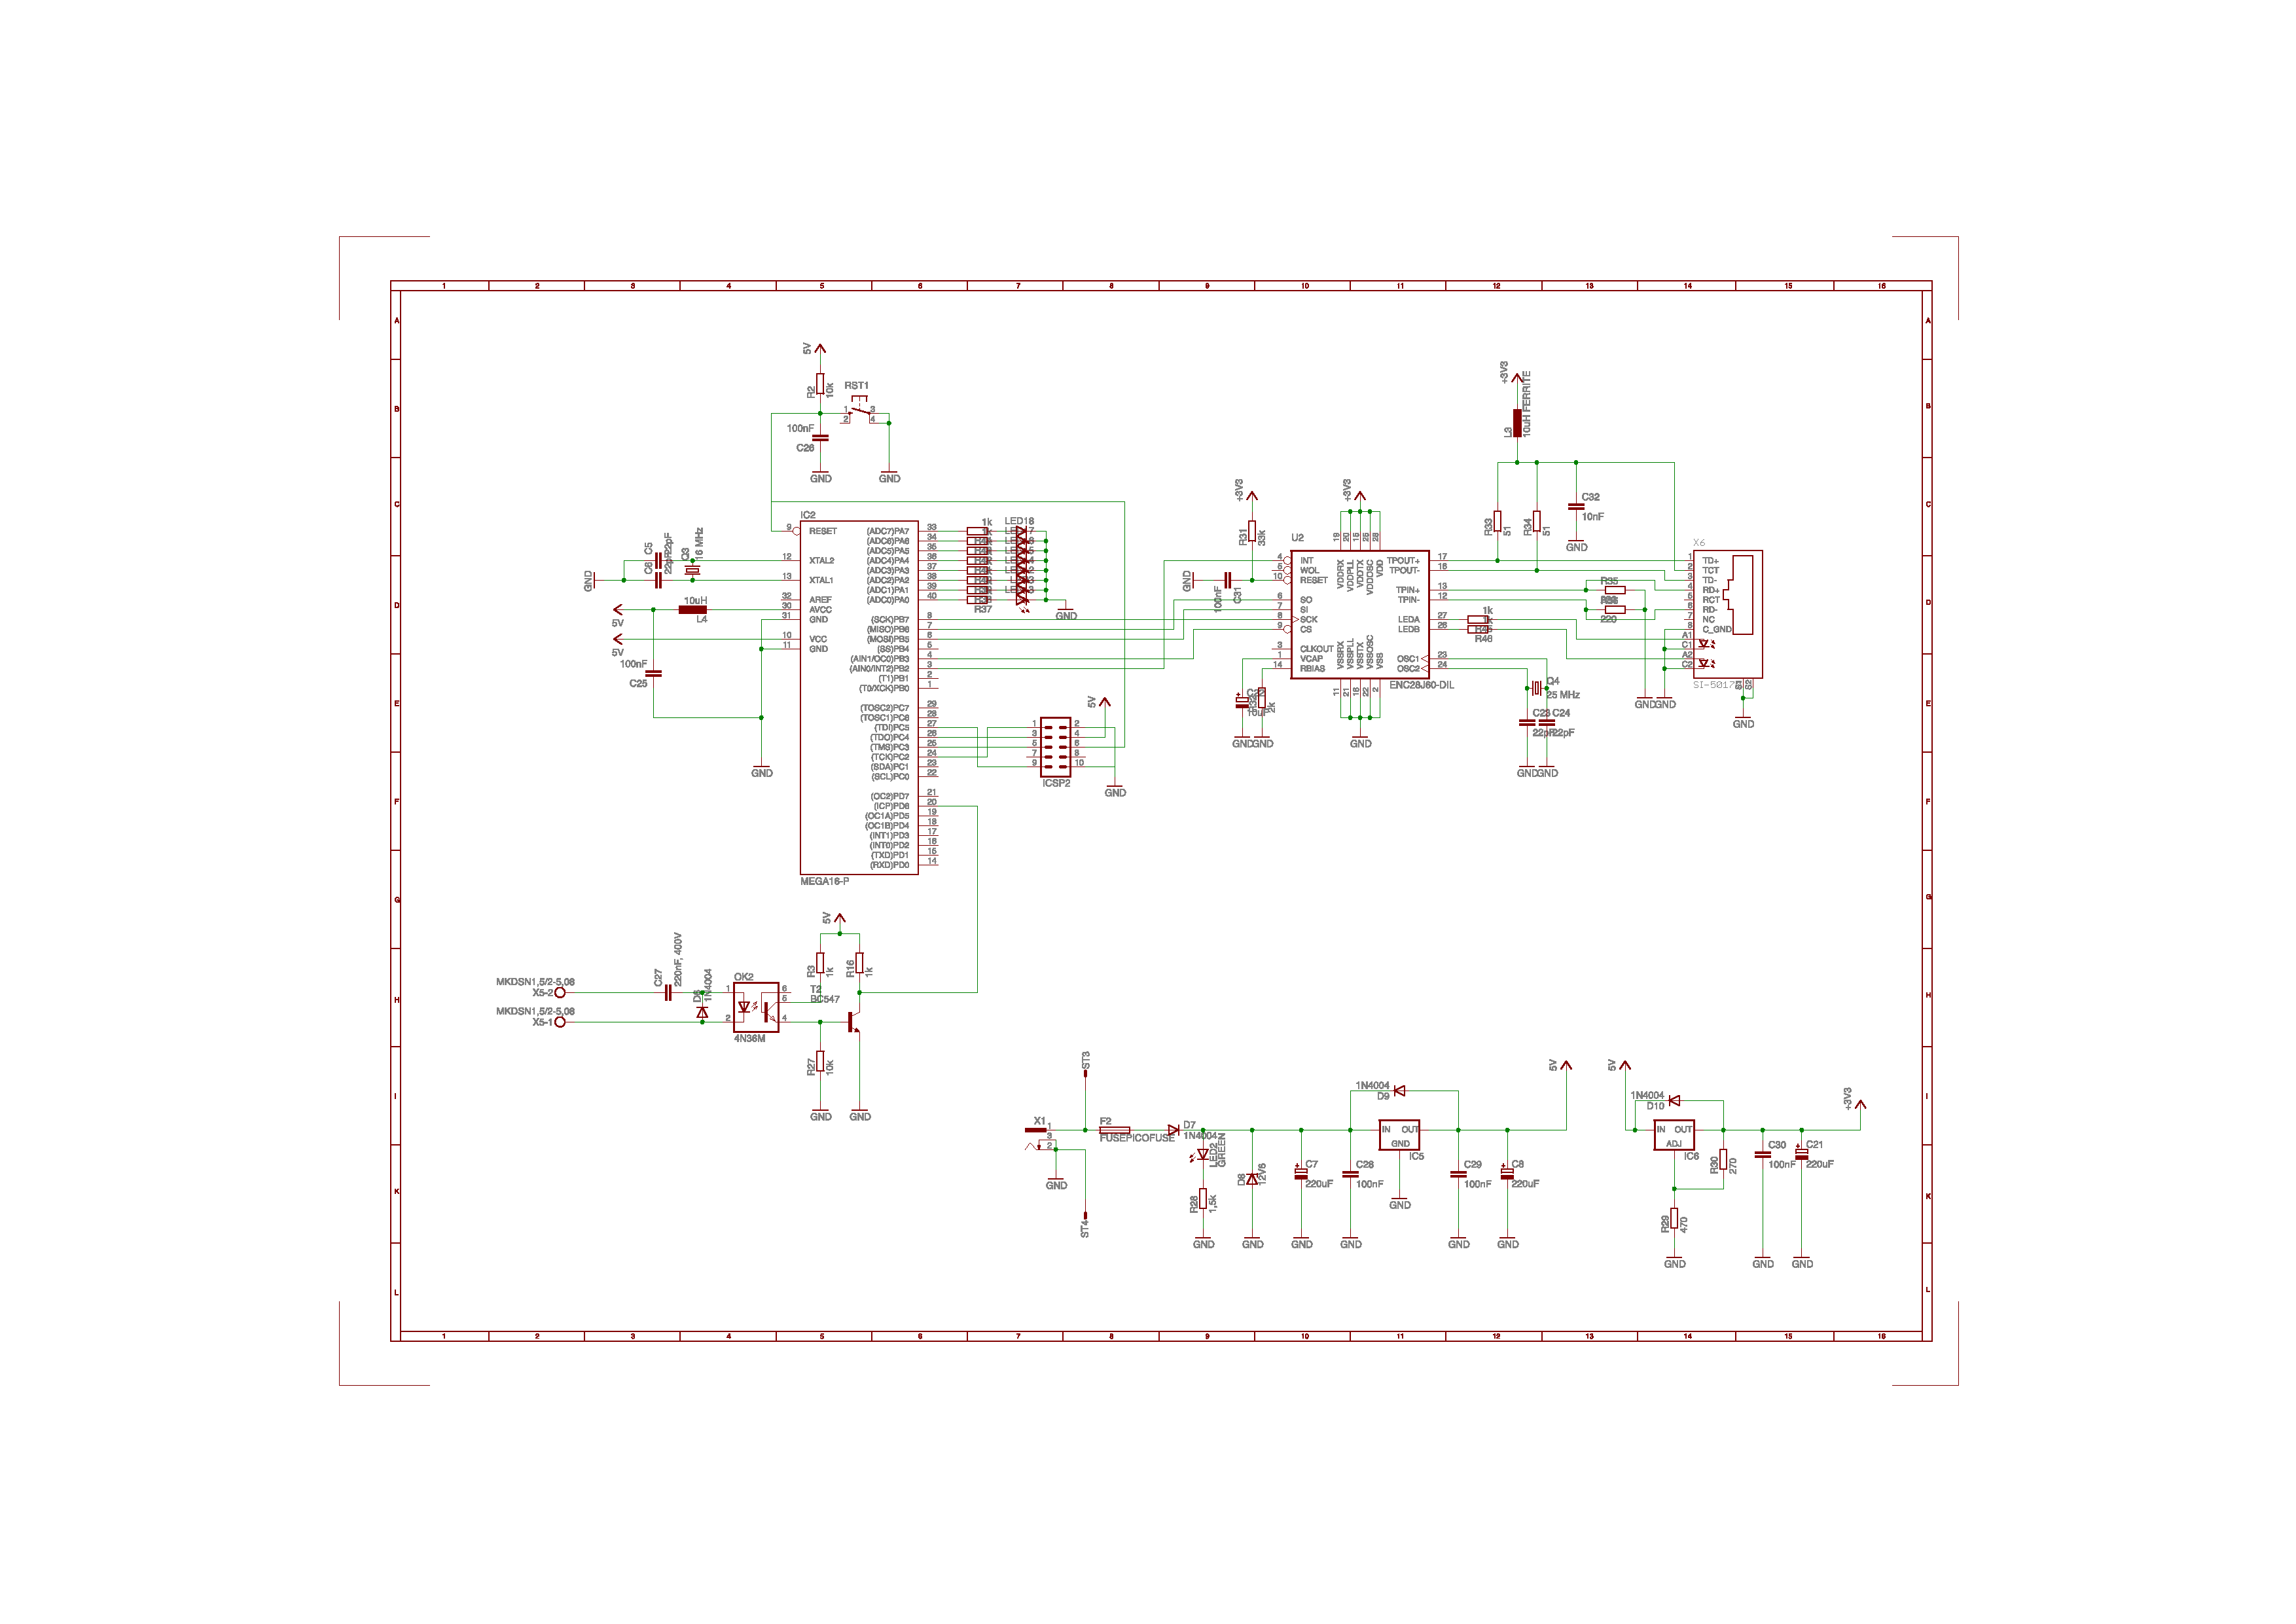
\includepdf[pages=-, landscape]{./pictures/eagle/bachelorarbeit.pdf}
\end{landscape}


%%%%%%%%%%%%%%%%%%%%%%%%%%%%%%%%%%%%%%%%%%%%%%%%%%%%%%%%%%%%%%%%%%%%%%%%%%%%%%%
\begin{landscape}
	\begin{multicols}{2}
		\chapter{Anhang}\label{anhang:software}

		Der Firmware-Code befindet sich in mehreren Verzeichnissen, damit er strukturell noch übersichtlicher ist und die Firmware in Zukunft noch leichter weiter entwickelt werden kann. Unter dem \textit{board}-Verzeichnis befindet sich die Header-Datei, in der die PIN-Belegungen des entworfenen Boards definiert wird. Die Definition des Registers des ATMega16-Mikrocontrollers und des ENC28J60-Mikrochips sind unter dem Verzeichnis \textit{device} zu finden. Die geschriebenen Treiber befinden sich unter dem Verzeichnis \textit{driver}. Um die Zeitmessungswerte zu puffern, gibt es einen \textit{Ringpuffer} im \textit{lib}-Verzeichnis. Schlussendlich stehen die nützliche Definitionen wie \textit{boolean}-Werte und \textit{NULL-Pointer}, falls sie im Compiler nicht definiert ist, im \textit{include}-Verzeichnis zur Verfügung. Die Gesamtstruktur ist in der folgenden Liste zu lesen: \\ \\ \\ \\

		\inputminted[fontsize=\scriptsize]{text}{./code/firmware/README}
		%\input{./code/firmware/firmware}
		\end{multicols}
\end{landscape}

\newpage

\begin{landscape}
Der Firmware-Code und der UNIX-Dämon-Code ist als Open Source Software unter der \textbf{BSD}-Lizenz\footnote{ist eine Lizenz für freie Software. Solche Software darf kostenfrei auch für kommerzielle Zwecke verwendet, verändert und vertrieben werden.} lizenziert bzw. veröffentlicht: \\

\inputminted{text}{./code/LICENSE}
%\input{./code/LICENSE}
\end{landscape}

\newpage

\begin{landscape}
	\begin{multicols}{2}
		\section{Firmware-Code}
		\subsubsection*{main-Programm}
		\subsubsection*{main.c}
		\inputminted[fontsize=\scriptsize,linenos,tabsize=4]{c}{./code/firmware/main.c}

		%%% board %%%
		\subsection*{board-Verzeichnis}
		\subsubsection*{freq.h}
		\inputminted[fontsize=\scriptsize,linenos,tabsize=4]{c}{./code/firmware/board/freq.h}

		%%% device %%%
		\subsection*{device-Verzeichnis}
		\subsubsection*{atmega16.h}
		\inputminted[fontsize=\scriptsize,linenos,tabsize=4]{c}{./code/firmware/device/atmega16.h}

		\subsubsection*{enc28j60.h}
		\inputminted[fontsize=\scriptsize,linenos,tabsize=4]{c}{./code/firmware/device/enc28j60.h}

		%%% driver %%%
		\subsection*{driver-Verzeichnis}
		\subsubsection*{enc28j60.c}
		\inputminted[fontsize=\scriptsize,linenos,tabsize=4]{c}{./code/firmware/driver/enc28j60.c}

		\subsubsection*{icp.h}
		\inputminted[fontsize=\scriptsize,linenos,tabsize=4]{c}{./code/firmware/driver/icp.h}

		\subsubsection*{icp.c}
		\inputminted[fontsize=\scriptsize,linenos,tabsize=4]{c}{./code/firmware/driver/icp.c}

		\subsubsection*{leds.h}
		\inputminted[fontsize=\scriptsize,linenos,tabsize=4]{c}{./code/firmware/driver/leds.h}

		\subsubsection*{leds.c}
		\inputminted[fontsize=\scriptsize,linenos,tabsize=4]{c}{./code/firmware/driver/leds.c}

		\subsubsection*{net.h}
		\inputminted[fontsize=\scriptsize,linenos,tabsize=4]{c}{./code/firmware/driver/net.h}

		\subsubsection*{net.c}
		\inputminted[fontsize=\scriptsize,linenos,tabsize=4]{c}{./code/firmware/driver/net.c}

		\subsubsection*{spi.h}
		\inputminted[fontsize=\scriptsize,linenos,tabsize=4]{c}{./code/firmware/driver/spi.h}

		\subsubsection*{spi.c}
		\inputminted[fontsize=\scriptsize,linenos,tabsize=4]{c}{./code/firmware/driver/spi.c}

		\subsubsection*{timer0.h}
		\inputminted[fontsize=\scriptsize,linenos,tabsize=4]{c}{./code/firmware/driver/timer0.h}

		\subsubsection*{timer0.c}
		\inputminted[fontsize=\scriptsize,linenos,tabsize=4]{c}{./code/firmware/driver/timer0.c}

		%%% include %%%
		\subsection*{include-Verzeichnis}
		\subsubsection*{common.h}
		\inputminted[fontsize=\scriptsize,linenos,tabsize=4]{c}{./code/firmware/include/common.h}

		\subsubsection*{stdbool.h}
		\inputminted[fontsize=\scriptsize,linenos,tabsize=4]{c}{./code/firmware/include/stdbool.h}

		%%% lib %%%
		\subsection*{lib-Verzeichnis}
		\subsubsection*{buffer.h}
		\inputminted[fontsize=\scriptsize,linenos,tabsize=4]{c}{./code/firmware/lib/buffer.h}

		\subsubsection*{buffer.c}
		\inputminted[fontsize=\scriptsize,linenos,tabsize=4]{c}{./code/firmware/lib/buffer.c}

		%%% Makefile %%%
		\subsection*{Makefile(s)}
		\subsubsection*{BSDmakefile}
		\inputminted[fontsize=\scriptsize,linenos,tabsize=4]{c}{./code/firmware/BSDmakefile}

		\subsubsection*{GNUmakefile}
		\inputminted[fontsize=\scriptsize,linenos,tabsize=4]{c}{./code/firmware/GNUmakefile}

		\subsubsection*{config.mk}
		\inputminted[fontsize=\scriptsize,linenos,tabsize=4]{c}{./code/firmware/config.mk}

		\subsubsection*{Makefile.mk}
		\inputminted[fontsize=\scriptsize,linenos,tabsize=4]{c}{./code/firmware/Makefile.mk}

		\subsubsection*{Makefile}
		\inputminted[fontsize=\scriptsize,linenos,tabsize=4]{c}{./code/firmware/Makefile}

		\newpage
		
		%%% UNIX daemon %%%
		\section{UNIX-Dämon}
		\subsection*{main-Programm}
		\subsubsection*{main.c}
		\inputminted[fontsize=\scriptsize,linenos,tabsize=4]{c}{./code/daemon/src/main.c}

		\subsection*{UDP-Protokoll}
		\subsubsection*{udp.h}
		\inputminted[fontsize=\scriptsize,linenos,tabsize=4]{c}{./code/daemon/src/udp.h}

		\subsubsection*{udp.c}
		\inputminted[fontsize=\scriptsize,linenos,tabsize=4]{c}{./code/daemon/src/udp.c}

		\subsection*{Fehlerbehandlung}
		\subsubsection*{error.h}
		\inputminted[fontsize=\scriptsize,linenos,tabsize=4]{c}{./code/daemon/src/error.h}

		\subsubsection*{error.c}
		\inputminted[fontsize=\scriptsize,linenos,tabsize=4]{c}{./code/daemon/src/error.c}

		%%% Makefile ??? %%%
		
	\end{multicols}
\end{landscape}
